\documentclass[UTF8]{article}
\usepackage{graphicx}
\usepackage{subfigure}
\usepackage{amsmath}
\usepackage{makecell}
\usepackage[utf8]{inputenc}
\usepackage[space]{ctex} %中文包
\usepackage{listings} %放代码
\usepackage{xcolor} %代码着色宏包
\usepackage{CJK} %显示中文宏包
\usepackage{float}

\definecolor{mygreen}{rgb}{0,0.6,0}
\definecolor{mygray}{rgb}{0.5,0.5,0.5}
\definecolor{mymauve}{rgb}{0.58,0,0.82}
\lstset{
	backgroundcolor=\color{white}, 
	basicstyle = \footnotesize,       
	breakatwhitespace = false,        
	breaklines = true,                 
	captionpos = b,                    
	commentstyle = \color{mygreen}\bfseries,
	extendedchars = false,
	frame = shadowbox, 
	framerule=0.5pt,
	keepspaces=true,
	keywordstyle=\color{black}\bfseries, % keyword style
	language = C++,                     % the language of code
	otherkeywords={string}, 
	numbers=left, 
	numbersep=5pt,
	numberstyle=\tiny\color{mygray},
	rulecolor=\color{black},         
	showspaces=false,  
	showstringspaces=false, 
	showtabs=false,    
	stepnumber=1,         
	stringstyle=\color{mymauve},        % string literal style
	tabsize=4,          
	title=\lstname           
}


%画图包
\usepackage{tikz}
%画图背景包
\usetikzlibrary{backgrounds}

%自定义命令
\newcommand{\psiG}{\psi_{G}}
%在tikz中画一个顶点
%#1:node名称
%#2:位置
%#3:标签
\newcommand{\newVertex}[3]{\node[circle, draw=black, line width=1pt, scale=0.8] (#1) at #2{#3}}
%在tikz中画一条边
\newcommand{\newEdge}[2]{\draw [black,very thick](#1)--(#2)}
%在tikz中放一个标签
%#1:名称
%#2:位置
%#3:标签内容
\newcommand{\newLabel}[3]{\node[line width=1pt] (#1) at #2{#3}}
\newcommand{\jumpLine} {\hspace*{\fill} \par}


\title{中国科学技术大学计算机学院\\《计算机系统概论》实验报告}
\author{}
\date{}

\begin{document}
\maketitle
	\begin{figure}[H]
		\centering
		
\includegraphics[width=2.5in]{xiaohui.jpg}\vspace{0.5cm}\\
		\large{
			实验题目:BINARY DIVISOR\\
			学生姓名:王章瀚\\
			学生学号:PB18111697\\
			完成日期:\today\\
		}\vspace{2cm}
		
		\large{计算机实验教学中心制\\2019年09月\\}
		\thispagestyle{empty}
		\clearpage  % 清除当页页码
	\end{figure}
	\newpage
	
	\section{实验要求}
	对给定有符号操作数,完成一个1-bit的右移算法。\par

	\section{设计思路}
	\subsection{思路一:移位寄存器法}
	对于右移的操作,可以使用移位寄存器的思路,将最高位补到最末位(第一次直接替换最后一位,因为右移后它不会存在的),并作15次\textbf{左移},最后补足最高位来完成。\par
	以4bit有符号数右移为例,如:$1101\rightarrow1011\rightarrow0110\rightarrow$最后补最高位成为1110\par
	用下表辅助说明:\par
	\begin{tabular}{|c|c|c|c|}
		\hline 
		& 执行前:R0 & 说明 & 执行后:R0 \\ 
		\hline 
		第1步 & 1101 & R0[4]==1 & 1101 \\ 
		\hline 
		第2步 & 1101 & R0[4]==1 & 1011 \\ 
		\hline 
		第3步 & 1011 & R0[4]==0 & 0110 \\ 
		\hline 
		第4步 & 0110 & R0原为负数 & 1110 \\ 
		\hline 
	\end{tabular} 
	
	
	\subsection{思路二:直接赋值法}
	也可以尝试直接把第n位的值赋给第(n-1)位。\par
	整体思路是利用两个寄存器,比如R1最开始保存x0001,R2最开始保存x0002。然后将R0与R2取与,可以知道R0上对应位是否为1,如果是1,则R4 += R1。然后将R1,R2左移,并循环该操作。直到R2为0,则完成,最后确认最高位即可。\par
	例如:\par
	\begin{tabular}{|c|c|c|c|c|c|}
		\hline 
		 & R0 & R1 & R2 & R4 & 说明\\ 
		\hline 
		第1步 & 1101 & 0001 & 0010 & 0000 & R0[1]==0 \\ 
		\hline 
		第2步 & 1101 & 0010 & 0100 & 0010 & R0[2]==1\\ 
		\hline 
		第3步 & 1101 & 0100 & 1000 & 0110 & R0[3]==1\\ 
		\hline 
		第4步 & 1101 & 1000 & 0000 & 1110 & R0为负数\\ 
		\hline 
	\end{tabular} 
	\jumpLine
	\jumpLine
	后面\textbf{3.2.2中}还会提到,这种方法中,由于R1,R2的使用有一定重复性,可以将两次循环并成1次(即R1和R2的作用不断互换),充分利用R1,R2的值的相关性来改进算法。\par
	此外,如果要追求极端的执行语句少,由于只有16位,可以复制15遍代码。经过测试,这样执行完x0000的右移,只需要58条指令。但这显然是\textbf{极为不妥}的,因此它占用了过大的内存空间。
	
	\section{关键代码讲解}
	\subsection{思路一:移位寄存器法}
	过程即按照前述思路进行。代码已注释好。\par
	最开始将R0的符号记录在R3里,而最后设置符号时,考虑了R0[15]现在为0,且R3记录了原本为1,才需要令R0[15]为1。\par
	这个代码执行对x8a9c的右移需要75条指令。\par
	对应代码如下:
	\begin{lstlisting}[language=C++, name=移位寄存器法(.hex)]
	0011000000000000	;		.ORIG	x3000
	0010001000010001	;		LD	R1, Nx000E	; serve as a counter
	0010011000010001	;		LD	R3, NxFFFE	; set R[0] to 0
	0101000000000011	;		AND	R0, R0, R3
	0010011000010000	;		LD	R3, Nx8000
	0101011000000011	;		AND	R3, R0, R3
	0000011000000001	;		BRzp LOOP		; check the sign of R0
	0001000000100001	;		ADD	R0, R0, #1
	0001000000000000	; LOOP	ADD	R0, R0, R0	; shift left
	0000011000000001	;		BRzp ZP
	0001000000100001	;		ADD	R0, R0, #1	; if R[15] is 1, R[0] <- 1
	0001001001111111	; ZP	ADD	R1, R1, #-1
	0000001111111011	;		BRp	LOOP
	0101000000000000	;		AND	R0, R0, R0
	0000100000000011	;		BRn	OK
	0101011011000011	;		BRzp R3, R3, R3
	0000011000000001	;		BRzp OK
	0001000000000011	;		ADD	R0, R0, R3	; these set the sign of R0
	1111000000100101	; OK	HALT
	0000000000001110	;		.FILL	x000E	
	1111111111111110	;		.FILL	xFFFE	
	1000000000000000	;		.FILL	x8000	
	
	\end{lstlisting}
	
	\subsection{思路二:直接赋值法}
	\subsubsection{原始思路}
	过程相对简单,即按照前述思路进行。代码已注释好。\par
	其中比较不易理解的地方是最后的设置符号。由于到了最后R1必然是x8000,因此可以将它与R0取与,这样R1就得到了R0[15]的值,然后往R4加即可\par
	这个代码执行对x8a9c的右移需要88条指令。\par
	\begin{lstlisting}[language=C++, name=直接赋值法(.bin)]
	0011000000000000	; 		begin at x3000.
	0010001000001011	; 		LD R1, Nx0001
	0010010000001011	;		LD R2, Nx0002
	0101100100100000	; 		AND R4, R4, #0
	0101011000000010	;LOOP	AND R3, R0, R2	; labeled LOOP
	0000010000000001	; 		BRz ZERO
	0001100100000001	; 		ADD R4, R4, R1	
	0001001001000001	;ZERO	ADD R1, R1, R1	; labeled ZERO
	0001010010000010	; 		ADD R2, R2, R2
	0000101111111010	; 		BRnp LOOP
	0101001000000001	; 		AND R1, R0, R1	
	0001000100000001	; 		ADD R0, R4, R1	; to set the sign
	1111000000100101	; 		HALT
	0000000000000001	;Nx0001	.FILL	x0001	; labeled Nx0001
	0000000000000010	;Nx0002	.FILL	x0002	; labeled Nx0002	
	\end{lstlisting}\par
	\subsubsection{改进算法}
	但是上述思路执行的语句还比较多,观察可以发现,R1和R2的功能有些重复,可以想办法复用来减少语句数。我的解决方案是:将两次循环混成一次,以轮流使用R1和R2的功能。\par
	这样将需要的指令数减少到了73。\par
	因为只是自己尝试着做的拓展实验,就没按照hex来写,而是为方便实现,用了汇编:\par
	\begin{lstlisting}[language=C++, name=直接赋值法改良(.asm)]
			.ORIG		x3000
			LD		R1, Nx0001
			LD		R2, Nx0002
			AND		R4, R4, #0	;一些初始化
	; 这一段LOOP将前述方法两次循环综合为一次
	; 这样做的好处在于,每个运算阶段中R1或R2
	; 的自加,有且仅有一个需要做,省去了一条
	; 指令。
	LOOP	AND		R3, R0, R2	;循环体开始
			BRz		ZERO1		
			ADD		R4, R4, R1	;若该位是1,则对应位加1
	ZERO1	ADD		R1, R2, R2
			BRz		FINAL		;判断是否结束
			AND		R3, R0, R1
			BRz		ZERO2
			ADD		R4, R4, R2	;若该位是1,则对应位加1
	ZERO2	ADD		R2, R1, R1
	BRnp	LOOP				;循环体结束
	
	FINAL	AND		R2, R0, R2
			ADD		R0, R4, R2
	
			HALT
	
	Nx0001	.FILL		x0001
	Nx0002	.FILL		x0002
			.END	
	\end{lstlisting}\par
	
	\section{调试分析}
	\subsection{测试数据选取}
	这两种方法看起来容易出问题的就是正负号的判断。\par
	至于其他的运算上,都是经过一定的判断决定是否要不要加1,要不要移位等,并且除了首尾操作略有不同外,中间的操作都是一样的,如果有问题,必然已经呈现。所以一般一个输入成功,基本上其他的也不会失败。\par
	综合上述原因考虑,可以用x8a9c和x7564一正一负及x0000三个数据来测试。\par
	
	\subsection{测试数据:x8a9c}
	\subsubsection{移位寄存器法}
	\begin{figure}[H]
		\centering
		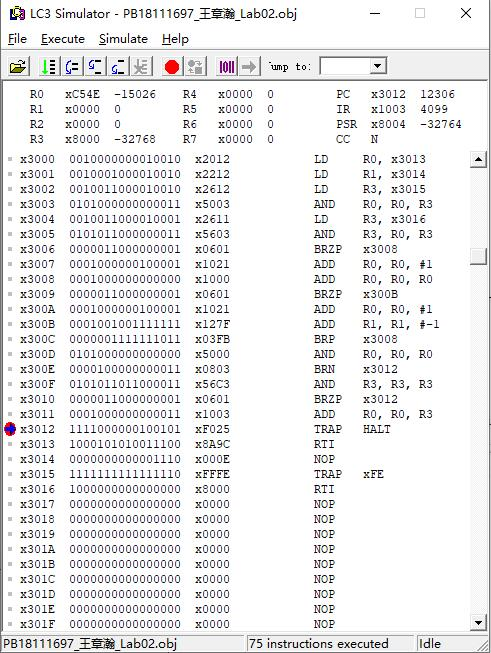
\includegraphics[width=0.4\linewidth]{x8a9c_1.jpg}
		\caption{移位寄存器法:x8a9c}
		\label{x8a9c_1}
	\end{figure}\par
	\subsubsection{直接赋值法}
	\begin{figure}[H]
		\begin{minipage}[H]{0.48\linewidth}
			\centering
			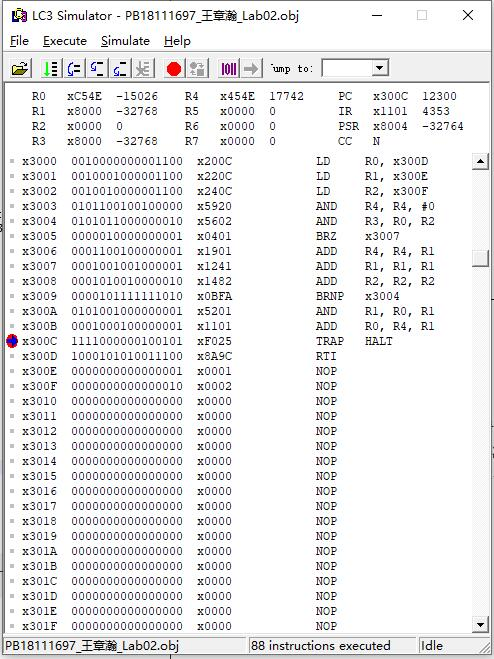
\includegraphics[scale=0.4]{x8a9c_2.jpg}
			\caption{直接赋值法:x8a9c}
			\label{x8a9c_2}
		\end{minipage}
		\qquad
		\begin{minipage}[H]{0.48\linewidth}
			\centering
			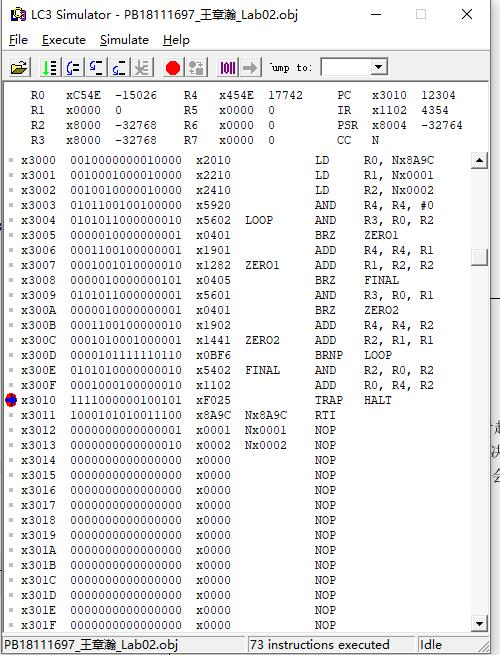
\includegraphics[scale=0.4]{x8a9c_3.jpg}
			\caption{改良的直接赋值法:x8a9c}
			\label{x8a9c_3}
		\end{minipage}
	\end{figure}

	\subsection{测试数据:x7564}
	\subsubsection{移位寄存器法}
	\begin{figure}[H]
		\centering
		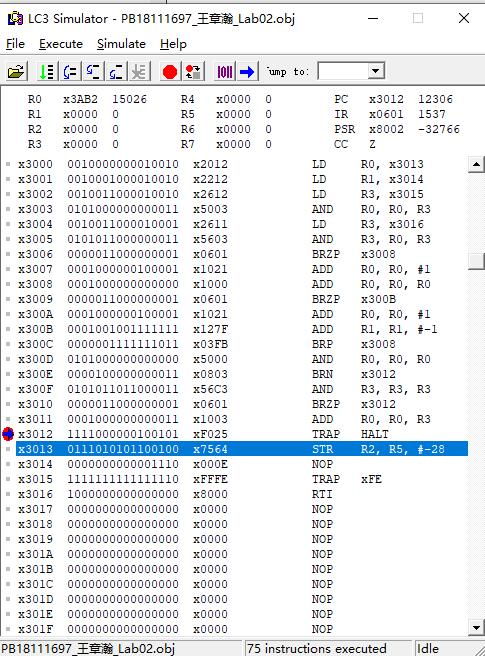
\includegraphics[width=0.4\linewidth]{x7564_1.jpg}
		\caption{移位寄存器法:x7564}
		\label{x7564_1}
	\end{figure}\par
	\subsubsection{直接赋值法}
	\begin{figure}[H]
		\begin{minipage}[H]{0.48\linewidth}
			\centering
			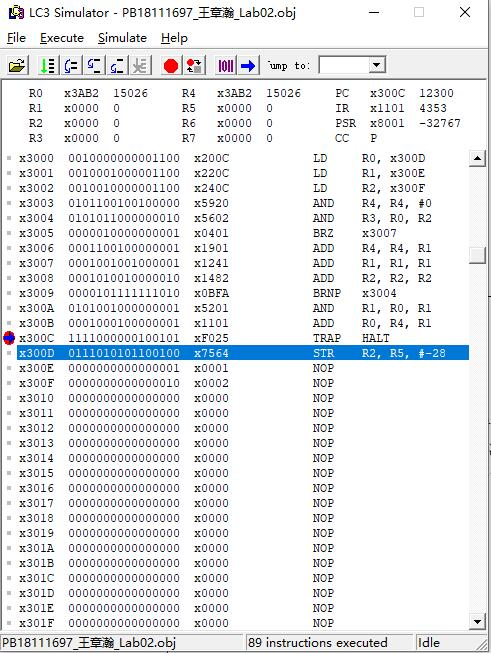
\includegraphics[scale=0.4]{x7564_2.jpg}
			\caption{直接赋值法:x7564}
			\label{x7564_2}
		\end{minipage}
		\qquad
		\begin{minipage}[H]{0.48\linewidth}
			\centering
			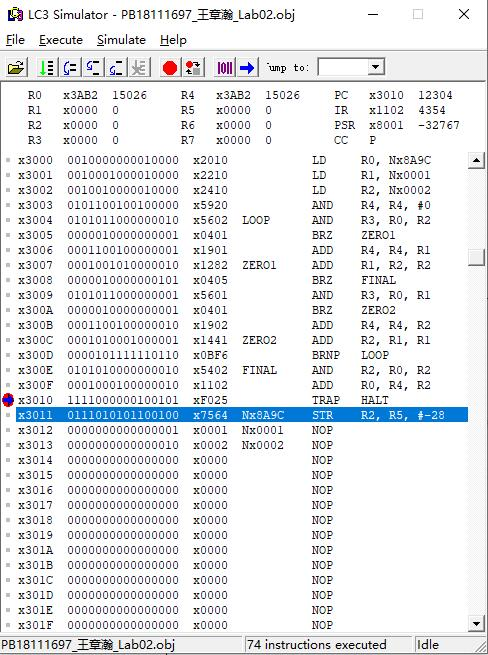
\includegraphics[scale=0.4]{x7564_3.jpg}
			\caption{改良的直接赋值法:x7564}
			\label{x7564_3}
		\end{minipage}
	\end{figure}
	
	\subsection{测试数据:x0000}
	\subsubsection{移位寄存器法}
	\begin{figure}[H]
		\centering
		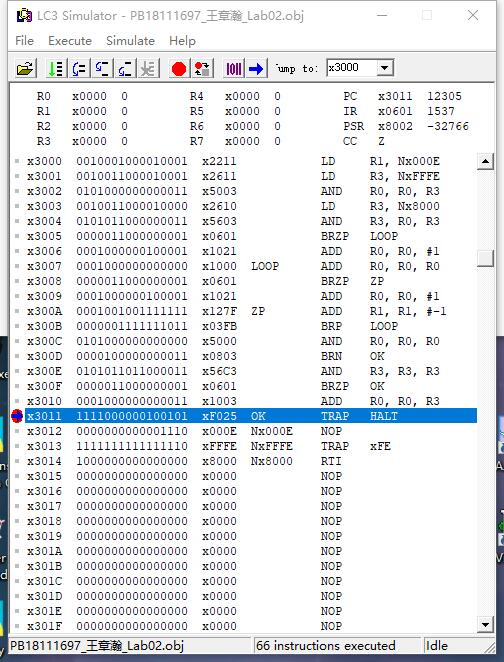
\includegraphics[width=0.4\linewidth]{x0000_1.jpg}
		\caption{移位寄存器法:x0000}
		\label{x0000_1}
	\end{figure}\par
	\subsubsection{直接赋值法}
	\begin{figure}[H]
		\begin{minipage}[H]{0.48\linewidth}
			\centering
			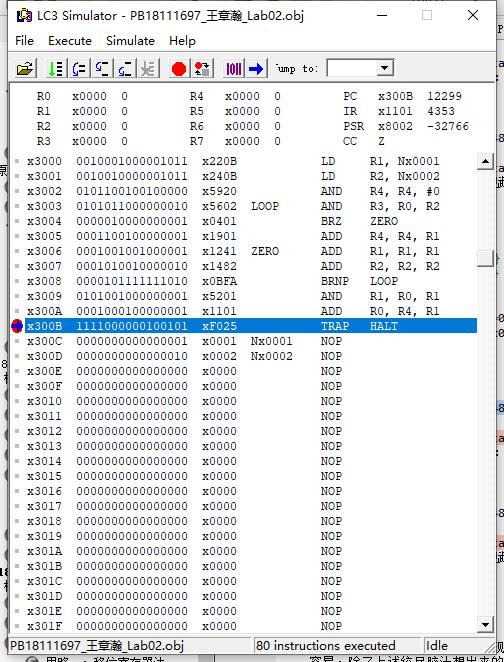
\includegraphics[scale=0.4]{x0000_2.jpg}
			\caption{直接赋值法:x0000}
			\label{x0000_2}
		\end{minipage}
		\qquad
		\begin{minipage}[H]{0.48\linewidth}
			\centering
			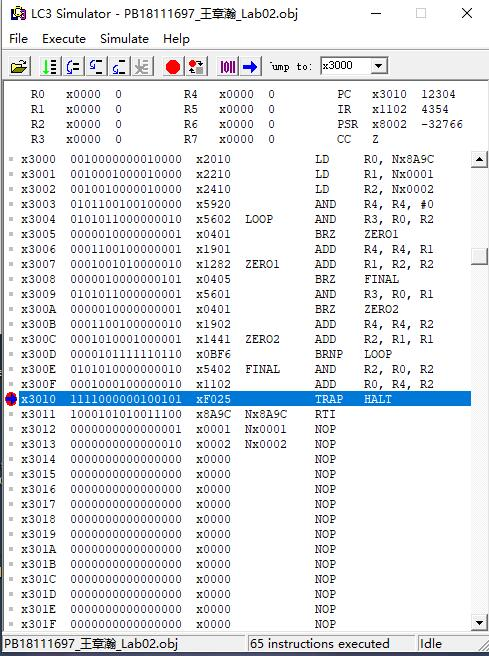
\includegraphics[scale=0.4]{x0000_3.jpg}
			\caption{改良的直接赋值法:x0000}
			\label{x0000_3}
		\end{minipage}
	\end{figure}
	
	\section{实验总结}
	本次实验对有符号16位操作数实现了右移操作,虽然看起来比较简单,但要实现出一个高效的算法实在不容易。\par
	就本人写的这几个代码来看,综合代码长度和执行效率,应该是\textbf{改良的直接赋值法}最佳。\par
	除了上述绞尽脑汁想出来的算法,我还听说过有人使用了一些表来实现等。总之实现右移的方法多种多样,但不论如何,似乎都不能避免这15到16次的循环,而每个循环也不容易压缩到小于5条指令。这可能也就是计算机不易做除法的原因之一吧。\par
	
	
	
\end{document}
